\setcounter{ExampleCounter}{1}
\begin{center}

\includegraphics[width=0.8\textwidth]{pacersNuggets}
\end{center}
Suppose you're doing some sort of study on players in the NBA.  You decide that rather than gathering data on \emph{all} NBA players, you can select a sample of, say, around 30 players.  In fact, you realize that since there are 30 teams, you can use stratified sampling and randomly select one player from each team.\\
\emph{Note: the data below is from the 2019-20 NBA season.}

\begin{center}
{\footnotesize
\begin{tabular}{l l c c l c c c r}
\textbf{Name} & \textbf{Team} & \textbf{No.} & \textbf{Age} & \textbf{Position} & \textbf{Height} & \textbf{Pts} & \textbf{Reb} & \textbf{Salary}\\
\hline
& & & & & & & \\
Jayson Tatum & Celtics & 0 & 22 & PF & 2.03 m & 23.4 & 7.0 & \$7,830,000\\
Joe Harris & Nets & 12 & 28 & SF & 1.98 m & 14.5 & 4.3 & \$7,666,667\\
RJ Barrett & Knicks & 9 & 20 & SG & 1.98 m & 14.3 & 5.0 & \$7,839,960\\
Ben Simmons & 76ers & 25 & 24 & PG & 2.08 m & 16.4 & 7.8 & \$8,113,930\\
Matt Thomas & Raptors & 21 & 26 & SG & 1.93 m & 4.9 & 1.5 & \$898,310\\
Daniel Gafford & Bulls & 12 & 21 & PF & 2.08 m & 5.1 & 2.5 & \$898,310\\
Andre Drummond & Cavaliers & 3 & 27 & C & 2.08 m & 17.7 & 15.2 & \$27,093,019\\
Langston Galloway & Pistons & 9 & 28 & SG & 1.85 m & 10.3 & 2.3 & \$7,333,333\\
Justin Holiday & Pacers & 8 & 31 & SF & 1.98 m & 8.3 & 3.3 & \$4,767,000\\
Khris Middleton & Bucks & 22 & 29 & SF & 2.01 m & 20.9 & 6.2 & \$30,603,448\\
Skal Labissiere & Hawks & 7 & 24 & PF & 2.08 m & 5.8 & 5.1 & \$2,338,847\\
PJ Washington & Hornets & 25 & 22 & PF & 2.01 m & 12.2 & 5.4 & \$3,831,840\\
KZ Okpala & Heat & 4 & 21 & SF & 2.03 m & 1.4 & 1.0 & \$898,310\\
Wes Iwundu & Magic & 25 & 25 & SF & 1.98 m & 5.8 & 2.5 & \$1,618,420\\
Rui Hachimura & Wizards & 8 & 22 & PF & 2.03 m & 13.5 & 6.1 & \$4,469,160\\
Andrew Wiggins & Warriors & 22 & 25 & SF & 2.01 m & 21.8 & 5.1 & \$27,504,630\\
Paul George & Clippers & 13 & 30 & SG & 2.03 m & 21.5 & 5.7 & \$30,560,700\\
Avery Bradley & Lakers & 11 & 29 & PG & 1.91 m & 8.6 & 2.3 & \$4,767,000\\
Jalen Lecque & Suns & 0 & 20 & PG & 1.93 m & 2.0 & 0.4 & \$898,310\\
Harry Giles III & Kings & 20 & 22 & C & 2.11 m & 6.9 & 4.1 & \$2,578,800\\
J.J. Barea & Mavericks & 5 & 36 & PG & 1.78 m & 7.7 & 1.8 & \$1,620,564\\
Bruno Caboclo & Rockets & 5 & 24 & SF & 2.06 m & 3.0 & 2.0 & \$1,845,301\\
Josh Jackson & Grizzlies & 20 & 23 & SG & 2.03 m & 9.0 & 3.1 & \$7,059,480\\
JJ Redick & Pelicans & 4 & 36 & SG & 1.91 m & 15.3 & 2.5 & \$13,486,300\\
Trey Lyles & Spurs & 41 & 24 & C & 2.06 m & 6.4 & 5.7 & \$5,500,000\\
Troy Daniels & Nuggets & 30 & 29 & SG & 1.93 m & 4.3 & 1.1 & \$384,541\\
Naz Reid & Timberwolves & 11 & 21 & C & 2.06 m & 9.0 & 4.1 & \$898,310\\
Luguentz Dort & Thunder & 5 & 21 & SG & 1.91 m & 6.8 & 2.3 & \$155,647\\
Jusuf Nurkic & Trail Blazers & 27 & 26 & C & 2.13 m & 17.6 & 10.3 & \$13,125,000\\
Donovan Mitchell & Jazz & 45 & 23 & SG & 1.85 m & 24.0 & 4.4 & \$3,625,760
\end{tabular}}
\end{center}

Now, how helpful is the table above?  How quickly can you glean information from it, or get an answer to a question you may have; for instance, if you wanted to have a sense of how diverse the salaries are in the NBA, would the list in the table above give you that?

It's unlikely that we can draw meaningful conclusions from a list of data like this; when we scan a table like this, there's no good way to aggregate the results that our eyes pass over.
\pagebreak

Because of this, much of statistics is concerned with describing and interpreting data in ways that we can quickly grasp.  In this section, we'll see how to use visual displays to do this; graphs are good because we can gather a lot of information at a glance.  In the next section, we'll discuss the use of numerical summaries, which are not quite as user-friendly as pictures, but more precise, and equally instructive once you know how to read them.  By using a combination of both approaches, we can get a full picture of a dataset like the one above.

\subsection{Types of Data}
Before we start summarizing data, we need to recognize that there are different types of data that need to be treated differently.  For instance, notice that one variable recorded above is the team that each player plays for, which cannot be treated the same way as their height, for instance.

If we wanted to compare players' heights, we could find the average, for instance.  This doesn't make any sense with their teams; we can't calculate an average, nor would it mean anything if we could.  This brings us to our first distinction: numerical versus categorical data.

\begin{formula}{Numerical and Categorical Data}
\paragraph{Numerical (or quantitative) data:} a quantitative variable is one that we count or measure.

\paragraph{Categorical (or qualitative) data:} a qualitative variable is one that divides items into categories.
\end{formula}

Notice that of the nine columns in the table, two of them are identifiers (name and jersey numbers) and thus not really variables that we're interested in summarizing.  You could certainly take the average of the jersey numbers, but what would that answer tell you?

We can break down the remaining seven columns into numerical and categorical variables:
\begin{center}
\begin{tabular}{l l}
\textbf{Variable} & \textbf{Type}\\
\hline
& \\
Team & Categorical\\
Age & Numerical\\
Position & Categorical\\
Height & Numerical\\
Points & Numerical\\
Rebounds & Numerical\\
Salary & Numerical
\end{tabular}
\end{center}

\paragraph{Note:} in case you're not familiar with positions in basketball, there are five players on the court for each team at any time: the point guard (PG), shooting guard (SG), small forward (SF), power forward (PF), and center (C), and the order listed roughly corresponds to the typical size of the players at each position (guards tend to be small and quick, and forwards and centers tend to be larger and stronger).

This distinction between numerical and categorical data is important because we will draw different types of graphs for the two different types.\\

There is another distinction within numerical data; notice that the definition above says that a numerical variable is one that we ``count or measure.''  It turns out that these two options distinguish two types of numerical data: discrete and continuous variables.

\begin{formula}{Discrete and Continuous Data}
\paragraph{Discrete variable:} a discrete variable is one that is counted, and it is limited to specific values.  For example, the number of children that a person has will always be a whole number; it cannot be anything in between.

\paragraph{Continuous variable:} a continuous variable is one that is measured; the values can be any number in a given range.  For example, a person's height can be measured as precisely as desired, so it's not limited to specific values.
\end{formula}

The line between discrete and continuous variables can sometimes be fuzzy.  For instance, is age a discrete or continuous variable in the NBA dataset?  You could make an argument either way.  Someone's age can be measured as precisely as desired, down to the minute or second or further, but as it is listed in the table (and usually written) it's given in terms of years, so it is limited to specific values (whole numbers).

The good news is that this distinction is not as crucial for us in this chapter; the work that we'll do with quantitative data will not change from discrete to continuous variables.  It is good to be aware of the distinction, but especially in fuzzy cases like age, don't spend too much time worrying about which category that variable falls into.\\

At this point, we're ready to start summarizing data with charts and graphs; for the examples that follow, we'll keep returning to the NBA dataset above.

\subsection{Dot Plots}
A dot plot is one of the simplest kinds of graphs, and it can be drawn for both numerical and categorical data.  We'll use the age of the NBA players as an example.

\begin{example}{Dot Plot}
Draw a dot plot to summarize the following data, the ages of 30 randomly chosen NBA players:
\[22, 28, 20, 24, 26, 21, 27, 28, 31, 29, 24, 22, 21, 25, 22,\]
\[25, 30, 29, 20, 22, 36, 24, 23, 36, 24, 29, 21, 21, 26, 23\]

\sol
To begin, draw an axis scaled to cover the full range of the data.  The age values range from 20 to 36, so our scale needs to extend at least that far.

\begin{center}
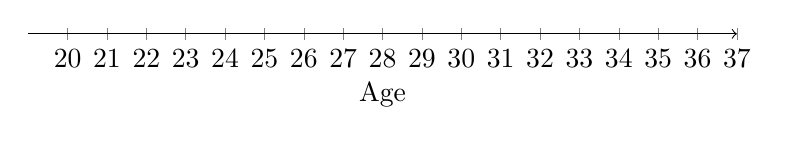
\begin{tikzpicture}
\begin{axis}[
    xmin=19, xmax=37,
    ymin=0, ymax=5,
    axis lines=center,
    axis on top=false,
    domain=0:1,
    x=0.5cm,
    y=0.02cm,
    xtick={19,20,...,37},
    xticklabels={19,20,...,37},
    axis y line=none,
    ytick={},
    yticklabels={},
    axis lines=middle,
    axis line style={->},
    x label style={at={(axis description cs:0.5,-5)},anchor=north},
    y label style={at={(axis description cs:-0.1,.5)},rotate=90,anchor=south},
    xlabel={Age},
    ylabel={},
    grid=none
    ]
\end{axis}
\end{tikzpicture}
\end{center}

Now, for each value in the dataset, place a dot at that position.  After placing the first seven values (22, 28, 20, 24, 26, 21, and 27), the graph looks like this:

\begin{center}
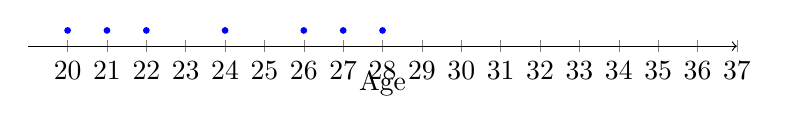
\begin{tikzpicture}
\begin{axis}[
    xmin=19, xmax=37,
    ymin=0, ymax=2,
    axis lines=center,
    axis on top=false,
    domain=0:1,
    x=0.5cm,
    y=0.2cm,
    xtick={19,20,...,37},
    xticklabels={19,20,...,37},
    axis y line=none,
    ytick={},
    yticklabels={},
    axis lines=middle,
    axis line style={->},
    x label style={at={(axis description cs:0.5,-0.5)},anchor=north},
    y label style={at={(axis description cs:-0.1,.5)},rotate=90,anchor=south},
    xlabel={Age},
    ylabel={},
    grid=none
    ]
	\addplot [blue,only marks,mark size=1] table {
	22 1
	28 1
	20 1
	24 1
	26 1
	21 1
	27 1
	};
\end{axis}
\end{tikzpicture}
\end{center}

At the eighth value, we encounter our first duplicate (28).  Simply place this dot above the one that is already placed at 28.  

\begin{center}
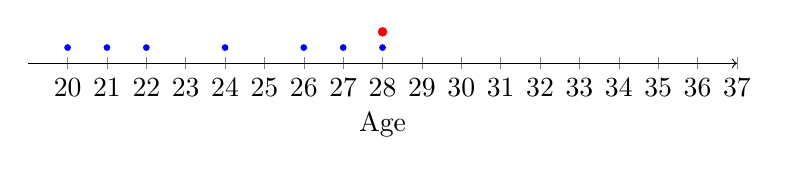
\begin{tikzpicture}
\begin{axis}[
    xmin=19, xmax=37,
    ymin=0, ymax=5,
    axis lines=center,
    axis on top=false,
    domain=0:1,
    x=0.5cm,
    y=0.2cm,
    xtick={19,20,...,37},
    xticklabels={19,20,...,37},
    axis y line=none,
    ytick={},
    yticklabels={},
    axis lines=middle,
    axis line style={->},
    x label style={at={(axis description cs:0.5,-0.5)},anchor=north},
    y label style={at={(axis description cs:-0.1,.5)},rotate=90,anchor=south},
    xlabel={Age},
    ylabel={},
    grid=none
    ]
	\addplot [blue,only marks,mark size=1] table {
	22 1
	28 1
	20 1
	24 1
	26 1
	21 1
	27 1
	};
	\addplot [red,only marks,mark size=1.5] table {
	28 2
	};
\end{axis}
\end{tikzpicture}
\end{center}

The final picture is shown below, after all the data is accounted for.

\begin{center}
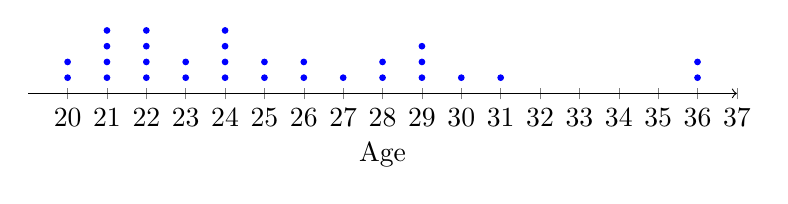
\begin{tikzpicture}
\begin{axis}[
    xmin=19, xmax=37,
    ymin=0, ymax=5,
    axis lines=center,
    axis on top=false,
    domain=0:1,
    x=0.5cm,
    y=0.2cm,
    xtick={19,20,...,37},
    xticklabels={19,20,...,37},
    axis y line=none,
    ytick={},
    yticklabels={},
    axis lines=middle,
    axis line style={->},
    x label style={at={(axis description cs:0.5,-0.5)},anchor=north},
    y label style={at={(axis description cs:-0.1,.5)},rotate=90,anchor=south},
    xlabel={Age},
    ylabel={},
    grid=none
    ]
	\addplot [blue,only marks,mark size=1] table {
	22 1
	28 1
	20 1
	24 1
	26 1
	21 1
	27 1
	28 2
	31 1
	29 1
	24 2
	22 2
	21 2
	25 1
	22 3
	25 2
	30 1
	29 2
	20 2
	22 4
	36 1
	24 3
	23 1
	36 2
	24 4
	29 3
	21 3
	21 4
	26 2
	23 2
	};
\end{axis}
\end{tikzpicture}
\end{center}
\end{example}

It's important as we start adding duplicate values that we space these dots evenly so that we can see at a glance where the grouping of the data occurs.  

\begin{try}
Draw a dot plot for the NBA players' positions.
\end{try}
\pagebreak

What you'll see as we encounter other graph types in this section is that the primary goal of most of them is to visualize how data is arranged, where it is tightly grouped together and where it is spread out.  This is true for dot plots as well.

For instance, looking at the dot plot in the previous example, what jumps out is that most of the players are between the ages of 20 and 29; only four of the players are 30 or older, and only two of them are older than 31.  Those two oldest players, at 36, are examples of what we often call \emph{outliers}, which are data points that are isolated from the main cluster of points.

\paragraph{Limitations:} a dot plot is designed to handle relatively small amounts of data; they are tedious to build and hard to read for large datasets.  For the dataset in the example, with 30 observations, a dot plot is a good way to get a quick glimpse of the data arrangement.

\subsection{Frequency Distributions}
The next tool, a frequency distribution or frequency table, is actually just another form of a dot plot.  Rather than drawing a dot for each individual value, though, a frequency table simply counts the \textbf{frequency} of each value, or how many times it occurs.

For instance, in the example of the NBA players' ages, there are two players aged 20, four at 21, and so on.  Continuing the pattern, we can build the table below.
\begin{center}
\begin{tabular}{c c}
\textbf{Age} & \textbf{Frequency}\\
\hline
& \\
20 & 2\\
21 & 4\\
22 & 4\\
23 & 2\\
24 & 4\\
25 & 2\\
26 & 2\\
27 & 1\\
28 & 2\\
29 & 3\\
30 & 1\\
31 & 1\\
32 & 0\\
33 & 0\\
34 & 0\\
35 & 0\\
36 & 2
\end{tabular}
\end{center}

In a frequency table, the first column lists the variable that we're summarizing and all the values of the variable that appear in our dataset; the second column lists the corresponding frequency for each value (note that the frequencies should all add up to 30, the size of the full dataset).  

Notice that there were several missing values (from 32 to 35), but we included them in the table anyway, and recorded zeros for the frequency.  This is mostly a matter of preference; some would remove those empty rows.  However, since our goal is to visualize how the data clusters and spreads out, those rows give the same sense that we got from the dot plot, that the two players at 36 are unusual within our dataset.

Frequency tables often include a third column, which contains the \textbf{relative frequency}.

\begin{formula}{Relative Frequency}
The \textbf{relative frequency} of a value is the proportion (or percentage) of its frequency to the total size of the dataset.

\paragraph{Note:} the relative frequencies of all values will always add up to 1 (although because of rounding, this may not always appear to be true).
\end{formula}

For instance, the first age, 20, appears twice in the full dataset, so its relative frequency is 2 out of 30, which could be simplified to 1 out of 15 (but generally we don't simplify these fractions) or written as a decimal (0.067) or percentage (6.7\%).  Any of these representations is perfectly acceptable.
\pagebreak

If we add this column to the frequency table, we get the following:
\begin{center}
\begin{tabular}{c c c}
\textbf{Age} & \textbf{Frequency} & \textbf{Relative Frequency}\\
\hline
& & \\
20 & 2 & 2/30 or 0.067\\
21 & 4 & 4/30 or 0.133\\
22 & 4 & 4/30 or 0.133\\
23 & 2 & 2/30 or 0.067\\
24 & 4 & 4/30 or 0.133\\
25 & 2 & 2/30 or 0.067\\
26 & 2 & 2/30 or 0.067\\
27 & 1 & 1/30 or 0.033\\
28 & 2 & 2/30 or 0.067\\
29 & 3 & 3/30 or 0.100\\
30 & 1 & 1/30 or 0.033\\
31 & 1 & 1/30 or 0.033\\
32 & 0 & 0/30 or 0.000\\
33 & 0 & 0/30 or 0.000\\
34 & 0 & 0/30 or 0.000\\
35 & 0 & 0/30 or 0.000\\
36 & 2 & 2/30 or 0.067
\end{tabular}
\end{center}

\begin{example}[https://www.youtube.com/watch?v=VQhKtct3nog]{Daily Commute}
Nineteen people were asked how many miles, to the nearest mile, they commute to work each day. They responded as follows: \[2, 5, 7, 3, 2, 10, 18, 15, 20, 7, 10, 18, 5, 12, 13, 12, 4, 5, 10.\] This is summarized in the frequency table below:

\begin{center}
\begin{tabular}{c | c | c}
\textbf{Data Value} & \textbf{Frequency} & \textbf{Relative Frequency}\\
\hline
3 & 3 & 3/19 \\
4 & 1 & 1/19 \\
5 & 3 & 3/19 \\
7 & 2 & 2/19 \\
10 & 3 & 4/19 \\
12 & 2 & 2/19 \\
13 & 1 & 1/19 \\
15 & 1 & 1/19 \\
18 & 1 & 1/19 \\
20 & 1 & 1/19  
\end{tabular}
\end{center}

\begin{enumerate}[(a)]
\item Is the table correct? If it is not correct, what is wrong?\\

It is incorrect, because the frequency column sums to 18, not 19 as it should.  One of the data values was left out.  Besides, two people responded that they commute 2 miles, and that doesn't appear on the table at all.\\

\item True or false: Three of the people surveyed commute three miles. If the statement is not correct, what should it be? If the table is incorrect, make the corrections.\\

False.  The frequency for 3 miles should be 1.  When building the table, the two that responded 2 miles got lumped into the 3 category.\\

\item What fraction of the people surveyed commute five or seven miles?\\

5/19\\

\item What fraction of the people surveyed commute 12 miles or more? Less than 12 miles? Between 5 and 13 miles (not including those who commute exactly 5 or exactly 13 miles)?\\

7/19, 12/19, 7/19
\end{enumerate}
\end{example}
\pagebreak
\text{}
\vfill

We can also create frequency distributions for categorical data.

\begin{example}{Categorical Frequency Distribution}
Create a frequency table for the NBA players' positions from the dataset at the beginning of this section, including a relative frequency column.

\sol
Since there are five possible results for position, we can start the table by creating the first column with these five values.  Then simply count the frequency of each position and record the result; the results are below.
\begin{center}
\begin{tabular}{c c c}
\textbf{Position} & \textbf{Frequency} & \textbf{Relative Frequency}\\
\hline
& & \\
PG & 4 & 13.3\%\\
SG & 9 & 30.0\%\\
SF & 7 & 23.3\%\\
PF & 5 & 16.7\%\\
C & 5 & 16.7\%
\end{tabular}
\end{center}

Clearly, the most popular positions are in the middle of the list, shooting guards and small forwards.  This makes sense because these tend to be versatile players who can fill multiple roles, so teams are more likely to sign them.
\end{example}
\vfill

\subsection{Grouped Frequency Distributions}
What if we wanted to build a frequency distribution for average points in the NBA dataset?  Since there is very little, if any, repetition in the values, the resulting table would have a lot of columns with 0's or 1's in them, and it wouldn't give us any sense of the grouping of the data.

Instead, we can create a \textbf{grouped frequency distribution}, which counts the frequency of specific \emph{ranges} instead of specific \emph{values}.

For instance, suppose we split the values from 0 to 25 into \textbf{classes} that cover 5 points each.  The first class would cover everything from 0 to 5, the second from 5 to 10, and so on.
\vfill

\paragraph{Hold On!} You may have already spotted a potential problem.  What if someone averages exactly 5 points; in which category do we count them?  If the classes go from 0 to 5 and 5 to 10, the overlap causes a problem.  To fix this, we'll make the first class from 0 to \textbf{just less than 5}, so that if a player averages 4.9 points per game, he'll belong to the first class, and if he averages 5.0 points per game, he'll belong to the second class.

This is a very important point, because this is the most common error that students make in creating grouped frequency tables; be careful with this.\\
\vfill

Here are our classes:
\begin{center}
\begin{tabular}{c}
\textbf{Points per Game}\\
\hline
\\
$0.0 - 4.9$\\
$5.0 - 9.9$\\
$10.0 - 14.9$\\
$15.0 - 19.9$\\
$20.0 - 24.9$
\end{tabular}
\end{center}

There are, of course, values between 4.9 and 5.0, so instead of writing 4.9, we could also write ``less than 5.''  However, as long as we're only considering the first decimal point, this is clear enough that anyone reading it can understand that what we really mean is ``less than 5.''  If we counted two decimal places, we'd need to replace 4.9 with 4.99 to make ourselves clear.
\vfill
\text{}
\pagebreak

\begin{proc}{Choosing Classes}
When building a grouped frequency distribution, you'll usually have the freedom to choose how you want to separate the classes.  Here are some guidelines you should follow:
\begin{itemize}
\item Each class should be the same width.  Notice in the example above that each class was five units wide.  If not, the grouped frequency distribution would not give a clear picture of how the data is arranged.
\item Classes cannot overlap.
\item Avoid empty classes if possible.  This can occur if you choose to have too many classes.
\item Don't make open-ended classes.  For instance, in the example above we didn't make the last class ``20 and above,'' which would have been an open-ended class.  The reason not to do this is that it violates the first guideline about having all classes have the same width.
\end{itemize}
\end{proc}

To find the appropriate class width to use, you can start by deciding on the number of classes you want to use, and the class width is found by dividing the distance from the minimum to the maximum by the number of classes. 

\begin{formula}{Class Width}

\[\textrm{Class Width } = \dfrac{\textrm{Maximum - Minimum}}{\textrm{Number of Classes}}\]
Round UP to the next whole number.
\end{formula}

\begin{example}{Grouped Frequency Distribution}
Build a grouped frequency table for points per game for the NBA players dataset, using a class width of 5.

\sol
We already defined the classes; all that's left is to count the number of players that fall into each range:
\begin{center}
\begin{tabular}{c c c}
\textbf{Points per Game} & \textbf{Frequency} & \textbf{Relative Frequency}\\
\hline
 & & \\
$0.0 - 4.9$ & 5 & 16.7\%\\
$5.0 - 9.9$ & 11 & 36.7\%\\
$10.0 - 14.9$ & 5 & 16.7\%\\
$15.0 - 19.9$ & 4 & 13.3\%\\
$20.0 - 24.9$ & 5 & 16.7\%
\end{tabular}
\end{center}

The most common category by far is the range from 5 to 10 points (just less than 10, technically).  The other players are equally split among the other four categories.
\end{example}

\begin{try}
Create a grouped frequency distribution for the salaries of the NBA players in the same dataset, using a class width of \$5 million.
\end{try}

Remember that frequency distributions are really the same concept as dot plots; the results are displayed differently, but both basically show a list of categories and the count in each category.

Keep this in mind, because this trend will continue; all of the next three graph types present variations on this same theme.  As you'll see, this goal of visualizing how data is arranged--where it is clustered and where it is spread out--is a very popular one, so we have many tools to achieve it.
\pagebreak

\subsection{Histograms and Bar Charts}
We'll lump two of the types of graphs together, because they are very similar.  If you go back and look at the example of a dot plot at the beginning of this section, and you blur the picture, what you'll see is basically a series of bars rising up from a horizontal axis, and the height of each bar represents how many times that value appears (its frequency, in other words).

This is exactly what a histogram or bar chart does; it simply replaces the series of dots with a bar of corresponding height.  Generally, we'll start by building a frequency distribution, and then draw a bar for each row of the table.  Thus, a histogram/bar chart contains \emph{exactly} the same information as the corresponding frequency table; the only difference is how this information is expressed.  Histograms and bar charts are used because we'd often rather look at a picture of the grouping than read a list of numbers in a table and interpret them.

\paragraph{What's the difference?} Okay then, what differentiates a histogram from a bar chart?  The difference is what kind of data we're summarizing: numerical or categorical.  Remember that we can draw a dot plot or frequency table for both types.  However, we when draw a histogram/bar chart, we make a (relatively small) distinction between them.

Visually, the difference is subtle, but it's based on the difference in the way that we can think of these two types of data.  With numerical data, there's a natural transition from one category to the next (from the $0.0 - 4.9$ class to the $5.0 - 9.9$ class, for instance), so we draw the bars in an unbroken sequence, without gaps between them.  Categorical data, on the other hand, has no such smooth transition; there's a sharp break between categories (the Knicks and the Nets are completely distinct, with no blending from one to the other).  To visualize this, we draw the bars with gaps between them.

Other than this, there is no fundamental distinction between histograms and bar charts.\\

\begin{example}{Histogram}
Build a histogram for points per game in the NBA dataset, using grouped classes with a class width of 5.

\sol
We already built the frequency table for this one:
\begin{center}
\begin{tabular}{c c}
\textbf{Points per Game} & \textbf{Frequency}\\
\hline
& \\
$0.0 - 4.9$ & 5\\
$5.0 - 9.9$ & 11\\
$10.0 - 14.9$ & 5\\
$15.0 - 19.9$ & 4\\
$20.0 - 24.9$ & 5
\end{tabular}
\end{center}
Now all we have to do is represent this with a graph.  Note that we will always draw vertical bars in this book, but this is simply a matter of preference; you can find histograms and bar charts that are drawn horizontally as well.
\begin{center}
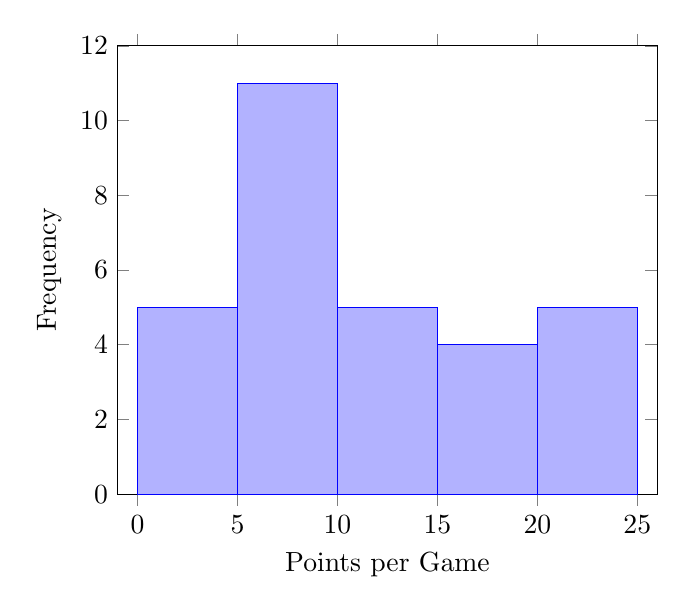
\begin{tikzpicture}
\begin{axis}[
	x tick label style={
		/pgf/number format/1000 sep=},
	ylabel={Frequency},
	xlabel={Points per Game},
	legend style={at={(0.5,-0.1)},
	anchor=north,legend columns=-1},
	ybar,
	bar width=15pt,
	ymin=0,
	ymax=12,
	xmin=-1,
	xmax=26,
	xtick=data,
	yticklabel style={
        /pgf/number format/fixed,
        /pgf/number format/precision=0
	},
	xticklabel style={
        /pgf/number format/fixed,
        /pgf/number format/precision=0
	},
]
\addplot+[ybar interval] plot 
	coordinates {(0,5) (5,11) (10,5)
		 (15,4) (20,5) (25,0) };
\end{axis}
\end{tikzpicture}
\end{center}
\end{example}

\begin{try}
Build a histogram for the players' ages in the NBA dataset.  There is no need to use grouping.
\end{try}

Note that although we don't show it in this section, we could also draw a histogram for the \emph{relative frequency}.  It turns out that the picture is identical, except that the vertical axis is relabeled; that's why we don't bother to cover that here.

Let's do an example with categorical data.

\begin{example}{Bar Chart}
Build a bar chart for the players' positions in the NBA dataset.

\sol
Remember that the reason we're calling this a bar chart is simply that position is a categorical variable rather than a numerical one.\\

Once again, we've already created the frequency table:
\begin{center}
\begin{tabular}{c c c}
\textbf{Position} & \textbf{Frequency}\\
\hline
& & \\
PG & 4\\
SG & 9\\
SF & 7\\
PF & 5\\
C & 5
\end{tabular}
\end{center}

Now, draw the bar chart (note the gaps between the bars):
\begin{center}
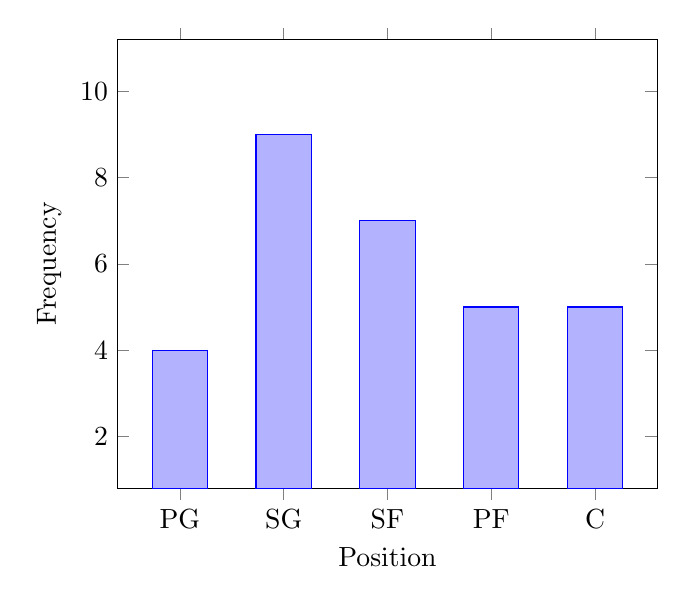
\begin{tikzpicture}
\begin{axis}[
	x tick label style={
		/pgf/number format/1000 sep=},
	ylabel={Frequency},
	xlabel={Position},
	xticklabels={,,PG,SG,SF,PF,C},
	yticklabels={,0,2,4,6,8,10},
	enlargelimits=0.15,
	legend style={at={(0.5,-0.1)},
	anchor=north,legend columns=-1},
	ybar,
	bar width=20pt,
	ymin=2,
	ymax=10,
	%nodes near coords,
	%nodes near coords style={
	%	/pgf/number format/.cd,fixed zerofill,precision=1},
	%nodes near coords align={vertical},
]
\addplot 
	coordinates {(1,4) (2,9)
		 (3,7) (4,5) (5,5)};
\end{axis}
\end{tikzpicture}
\end{center}
\end{example}

\subsection{Stem-and-Leaf Plots}
There is one major downside to grouped frequency distributions: some of the data gets lost in the summary.  In other words, maybe in an example all we know is that there are 10 observations between 20 and 25, but we don't know exactly what all those observations are.  This is an example of the trade-off between clarity and precision: often, the more precise we are, the less clear our summary will be.

To split the difference and display the data in a way that exhibits where it is clustered without losing any information about the data is to use a \textbf{stem-and-leaf} plot.  Here, the data is grouped by tens; each tens value is a stem, and all the data points that have that tens value are listed as the leaves.  We'll illustrate with an example.
\pagebreak

\begin{example}{Stem and Leaf Plot}
Suppose you gathered data on how long it took you to get ready in the morning.  For 40 days, you measured the amount of time between when your alarm went off and when you left the house.  The results are below, rounded to the nearest minute:
\begin{center}
\begin{tabular}{c c c c c c c c c c}
35 & 28 & 25 & 23 & 23 & 32 & 29 & 19 & 21 & 13\\
24 & 26 & 25 & 31 & 30 & 20 & 25 & 29 & 37 & 26\\
32 & 36 & 18 & 17 & 15 & 24 & 21 & 16 & 19 & 30\\
38 & 27 & 22 & 24 & 28 & 17 & 31 & 32 & 21 & 28\\
\end{tabular}
\end{center}
Build a stem-and-leaf plot for this data.

\sol
The tens places are 1, 2, and 3, and each of them gets a category:
\begin{center}
\begin{tabular}{r | l}
Stems & Leaves\\
\hline
1 & {\color{white}3 5 6 7 7 8 9 9}\\
2 & {\color{white}0 1 1 1 2 3 3 4 4 4 5 5 5 6 6 7 8 8 8 9 9}\\
3 & {\color{white}0 0 1 1 2 2 2 5 6 7 8}
\end{tabular}
\end{center}

Finally we go through (carefully) and find each value that begins with a 1 and list the ones place of each of them under the first category, and similarly with the other two categories.
\begin{center}
\begin{tabular}{r | l}
Stems & Leaves\\
\hline
1 & 3 5 6 7 7 8 9 9\\
2 & 0 1 1 1 2 3 3 4 4 4 5 5 5 6 6 7 8 8 8 9 9\\
3 & 0 0 1 1 2 2 2 5 6 7 8
\end{tabular}
\end{center}
\end{example}

Notice that we arranged the leaves in order; this isn't strictly necessary, but it makes the data a bit more orderly.

Once again, this stem-and-leaf plot illustrates where the data is clustered, as the length of each row of leaves is equivalent to the height of a bar on a histogram, but it does this without losing any information.  In other words, if we were simply given the stem-and-leaf plot, we could completely recreate the data set.\\

For three-digit data values (or longer), the leaves are usually still the last digits (the unit digits), and the stems are everything before that.  For instance, observe the data set below and the corresponding stem-and-leaf plot.

\begin{center}
\begin{tabular}{c c c c c c c c c c}
135 & 128 & 125 & 123 & 123 & 132 & 129 & 119 & 121 & 113\\
124 & 126 & 125 & 131 & 130 & 120 & 125 & 129 & 137 & 126\\
\end{tabular}
\end{center}

\begin{center}
\begin{tabular}{r | l}
Stems & Leaves\\
\hline
11 & 3 9\\
12 & 0 1 3 3 4 5 5 5 6 6 8 9 9\\
13 & 0 1 2 5 7
\end{tabular}
\end{center}

\begin{try}
Build a stem-and-leaf plot for the NBA players' rebounds per game, using the ones place as the stems and the tenths place as the leaves.
\end{try}
\vfill
\pagebreak

\subsection{Scatterplots}
The final type of graph that we'll consider, scatterplots are different from the rest; the rest are all concerned basically with frequency, although they simply display the results in different ways, and they can be used with either numerical or categorical data.  On the other hand, scatterplots are designed to compare one numerical variable to another, and we can use them to spot a connection or \emph{correlation} between the two.

For instance, in the NBA dataset, we may suspect that there is some relationship between the number of points per game that a player averages and his salary.  We'd expect to see that players who score more points are likely paid more.  Looking at the raw data in the table, there's no way to observe that, but if we draw a scatterplot, we can see whether our guess is correct.\\

To draw a scatterplot, we will call one of our variables $x$ and the other $y$.  It is worth understanding the distinction between the two, but the good news is that if we reverse the choice, the fundamental relationship isn't changed, and we can still do everything we'd like to.

\begin{formula}{Explanatory Variable}
When drawing a scatterplot, ask yourself this question:
\begin{center}
``Which variable determines the other?''
\end{center}
Your answer will be called the \textit{explanatory variable} and labeled as $x$.
\end{formula}

In our example, does it make more sense to say that the number of points a player scores determines his salary, or that his salary determines how many points he scores?  It should be clear that $x$ should represent points, and $y$ should thus represent salary.  Remember, though, if you reverse this, the basic relationship will still be evident.

To illustrate the process, let's use only the first 10 rows of the full dataset, for the sake of simplicity.  After labeling our variables, here's what we have:
\begin{center}
\begin{tabular}{c c}
\textbf{Pts ($x$)} & \textbf{Salary ($y$) in millions}\\
\hline
& \\
23.4 & 7.8\\
14.5 & 7.7\\
14.3 & 7.8\\
16.4 & 8.1\\
4.9 & 0.9\\
5.1 & 0.9\\
17.7 & 27.1\\
10.3 & 7.3\\
8.3 & 4.8\\
20.9 & 30.6
\end{tabular}
\end{center}

Now draw a grid with $x$ on the horizontal axis and $y$ on the vertical axis:
\begin{center}
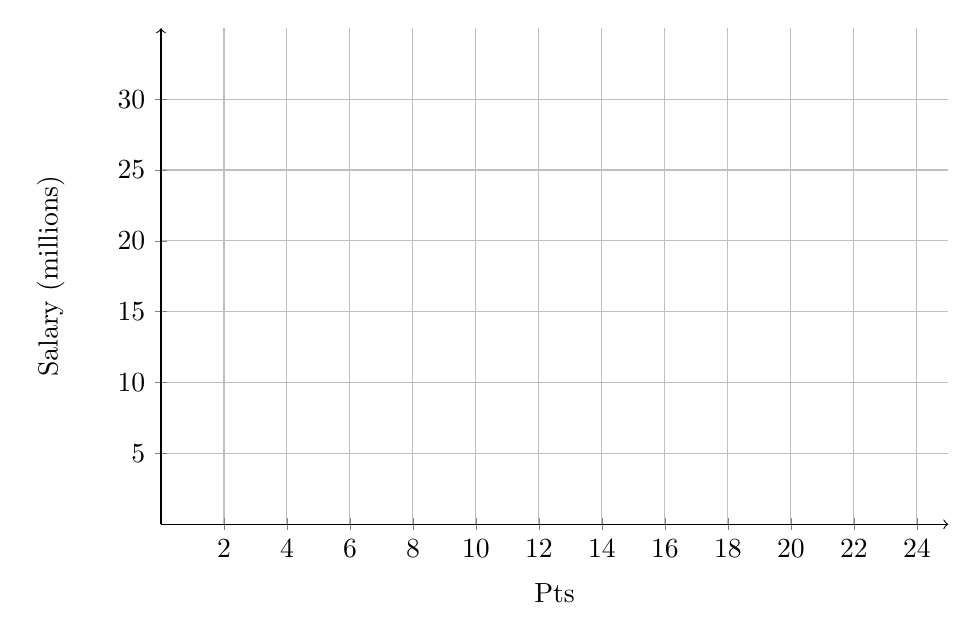
\begin{tikzpicture}
\begin{axis}[
    xmin=0, xmax=25,
    ymin=0, ymax=35,
    axis lines=center,
    axis on top=false,
    domain=0:1,
    x=0.4cm,
    y=0.18cm,
    xtick={2,4,...,24},
    xticklabels={2,4,...,24},
    ytick={0,5,...,30},
    yticklabels={0,5,...,30},
    axis lines=middle,
    axis line style={->},
    x label style={at={(axis description cs:0.5,-0.1)},anchor=north},
    y label style={at={(axis description cs:-0.11,.5)},rotate=90,anchor=south},
    xlabel={Pts},
    ylabel={Salary (millions)},
    grid=major
    ]
\end{axis}
\end{tikzpicture}
\end{center}
\pagebreak

Each row of the table will correspond to a dot on this grid; the horizontal position is defined by $x$, and the vertical position is defined by $y$.  For instance, the first dot will have a horizontal position of 23.4 and a vertical position of 7.8, which is shown below:
\begin{center}
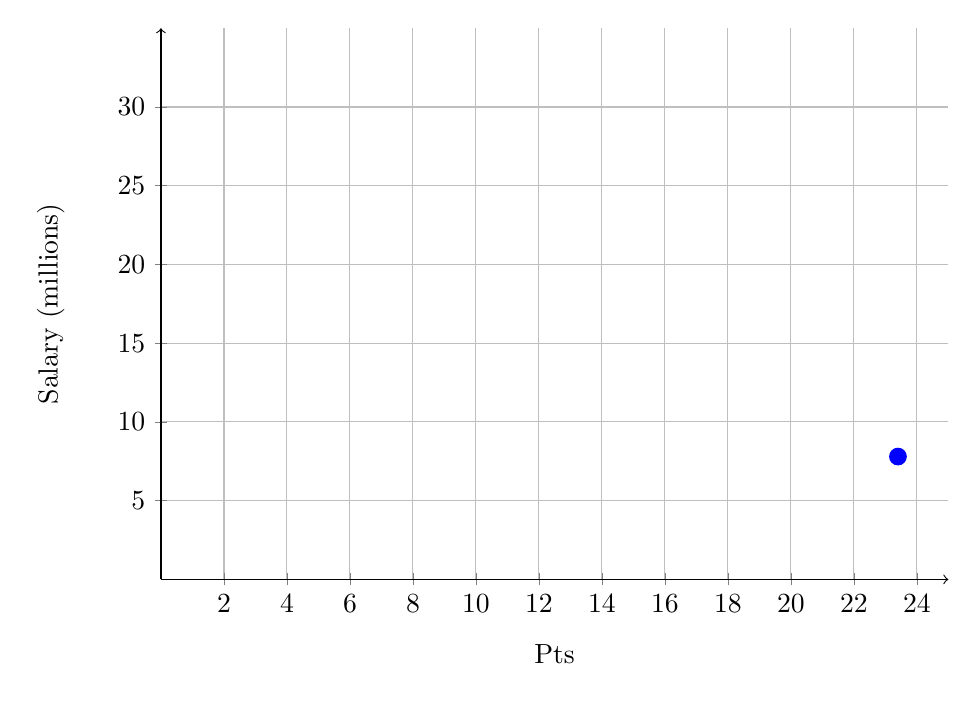
\begin{tikzpicture}
\begin{axis}[
    xmin=0, xmax=25,
    ymin=0, ymax=35,
    axis lines=center,
    axis on top=false,
    domain=0:1,
    x=0.4cm,
    y=0.2cm,
    xtick={2,4,...,24},
    xticklabels={2,4,...,24},
    ytick={0,5,...,30},
    yticklabels={0,5,...,30},
    axis lines=middle,
    axis line style={->},
    x label style={at={(axis description cs:0.5,-0.1)},anchor=north},
    y label style={at={(axis description cs:-0.11,.5)},rotate=90,anchor=south},
    xlabel={Pts},
    ylabel={Salary (millions)},
    grid=major
    ]
	\addplot [blue,only marks,mark size=3] table {
	23.4 7.8
	};
\end{axis}
\end{tikzpicture}
\end{center}

Notice that when we draw scatterplots by hand, the positions are all approximate, but since the goal is to get a big-picture view of the relationship between the two variables, that's okay.

Once we draw all the points, here is the final picture:
\begin{center}
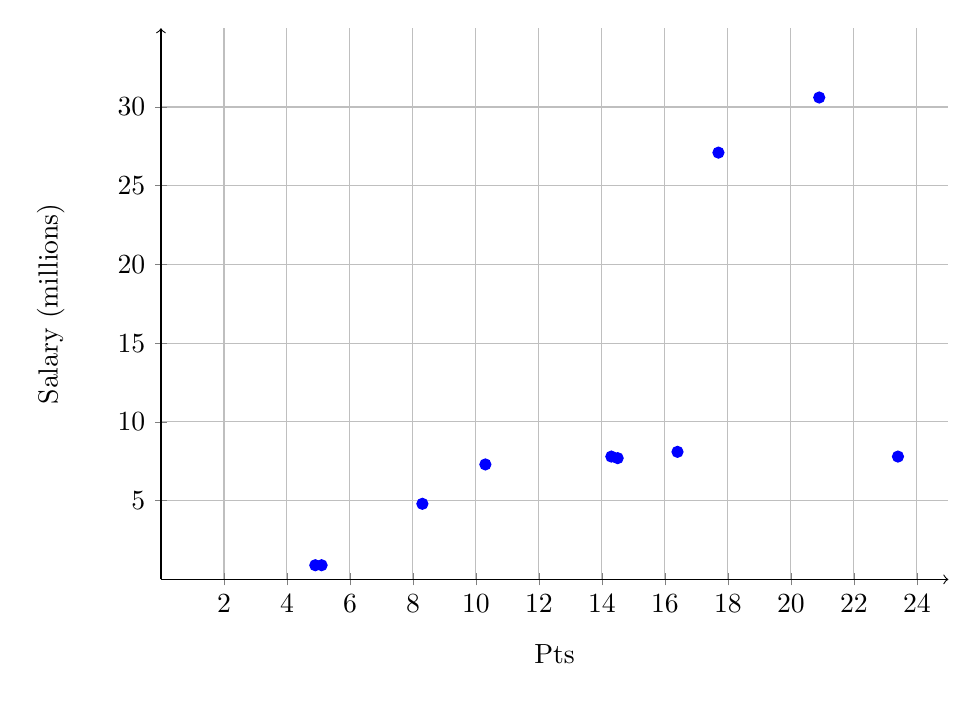
\begin{tikzpicture}
\begin{axis}[
    xmin=0, xmax=25,
    ymin=0, ymax=35,
    axis lines=center,
    axis on top=false,
    domain=0:1,
    x=0.4cm,
    y=0.2cm,
    xtick={2,4,...,24},
    xticklabels={2,4,...,24},
    ytick={0,5,...,30},
    yticklabels={0,5,...,30},
    axis lines=middle,
    axis line style={->},
    x label style={at={(axis description cs:0.5,-0.1)},anchor=north},
    y label style={at={(axis description cs:-0.11,.5)},rotate=90,anchor=south},
    xlabel={Pts},
    ylabel={Salary (millions)},
    grid=major
    ]
	\addplot [blue,only marks,mark size=2] table {
	23.4 7.8
	14.5 7.7
	14.3 7.8
	16.4 8.1
	4.9 0.9
	5.1 0.9
	17.7 27.1
	10.3 7.3
	8.3 4.8
	20.9 30.6
	};
\end{axis}
\end{tikzpicture}
\end{center}

Notice that yes, there is an overall trend toward higher scorers being paid more, but that is not an unyielding rule; for instance, the first player (Jayson Tatum) is the highest scorer in this smaller list, but he's not nearly the highest-paid player.  Clearly there are other factors at play (age, position, team, whether a player is still on his rookie contract, etc.).  This is often the case; scatterplots can hint at relationships, but there are often other unseen relationships at play.
\pagebreak

\begin{example}{Scatterplot: TV Price}
The following table shows, for a sample of Samsung LCD TVs, their size and their price.  Construct a scatterplot for this data.
\begin{center}
\begin{tabular}{c c | c c}
Size (in.) & Price (\$) & Size (in.) & Price (\$)\\
\hline
\\
43 & 500 & 60 & 1200\\
55 & 900 & 45 & 1600\\
51 & 900 & 19 & 200\\
32 & 400 & 55 & 2200\\
51 & 1200 & 60 & 1700\\
37 & 500 & 55 & 2000\\
60 & 2800 & 22 & 300\\
60 & 1100 & 40 & 600\\
46 & 1600 & 40 & 900
\end{tabular}
\end{center}

\sol
We could pick either variable to be $x$, but it makes more sense to say that the size of a TV determines its price than to say that the price of a TV determines its size.

The scatterplot below shows the relationship between the two.
\begin{center}
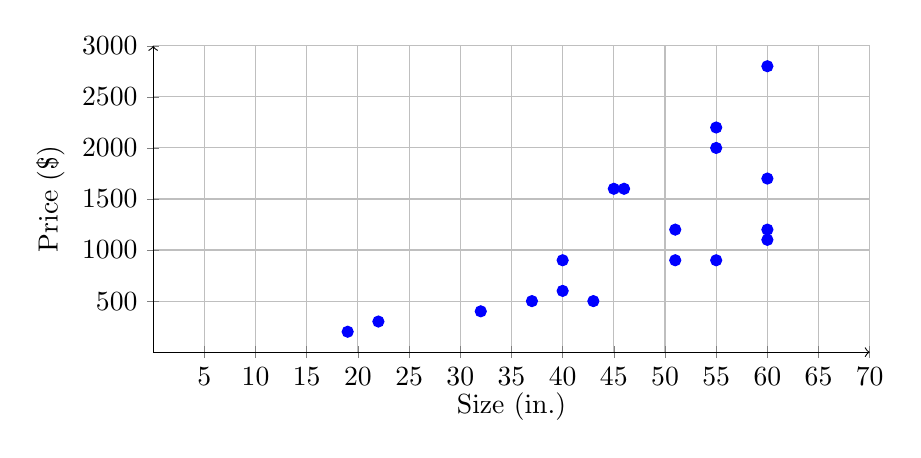
\begin{tikzpicture}
\begin{axis}[
    xmin=0, xmax=70,
    ymin=0, ymax=3000,
    axis lines=center,
    axis on top=false,
    domain=0:1,
    x=0.13cm,
    y=0.0013cm,
    xtick={5,10,...,70},
    xticklabels={5,10,...,70},
    ytick={0,500,...,3000},
    yticklabels={0,500,...,3000},
    axis lines=middle,
    axis line style={->},
    x label style={at={(axis description cs:0.5,-0.1)},anchor=north},
    y label style={at={(axis description cs:-0.11,.5)},rotate=90,anchor=south},
    xlabel={Size (in.)},
    ylabel={Price (\$)},
    grid=major
    ]
	\addplot [blue,only marks,mark size=2] table {
	43 500
	55 900
	51 900
	32 400
	51 1200
	37 500
	60 2800
	60 1100
	46 1600
	60 1200
	45 1600
	19 200 
	55 2200
	60 1700
	55 2000
	22 300
	40 600
	40 900
	};
\end{axis}
\end{tikzpicture}
\end{center}
\end{example}

Notice again that while there is a clear upward trend, meaning that larger TVs tend to be more expensive, there is plenty of variation, so there are other factors that play into the price, such as resolution or model.

\begin{try}
The following table shows a sample of homes on the market, recording their size in square feet and their price in thousands of dollars (so for instance, the first home is selling for \$400,000).
\begin{center}
\begin{tabular}{c | c}
Size (sq. ft.) & Selling Price (\$1000s)\\
\hline
\\
2521 & 400\\
2555 & 426\\
2735 & 428\\
2846 & 435\\
3028 & 469\\
3049 & 475\\
3198 & 488\\
3198 & 455\\
\end{tabular}
\end{center}

Construct a scatter plot for this data.
\end{try}
\vfill
\pagebreak

\subsection{Using Your Calculator}
On a TI graphing calculator, pressing \calcbutton{2ND} then \calcbutton{Y=} will open the statistics plots menu.
\begin{center}
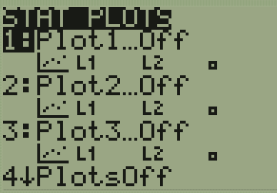
\includegraphics[width=2in]{AgeExample2}
\end{center}

You can draw multiple plots at once, but there's no need to here.  Pressing \calcbutton{ENTER} will open the first plot.  By default, statistics plots are turned off, so if we want to use one, we have to turn it on first.
\begin{center}
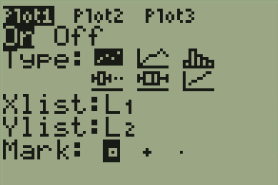
\includegraphics[width=2in]{AgeExample3}
\end{center}

Notice that there are six options for the type of plot, but only two of them match ones we've discussed in this section: the scatterplot and the histogram.  However, recall that dot plots, frequency distributions, and stem-and-leaf plots are all essentially equivalent to histograms, so we can use the histogram option to let the calculator handle the frequency counting for us, then we can draw the result however we like, as a table or graph.

\subsubsection{Histograms}
We'll use the NBA players' ages as an example (before continuing, enter the data by pressing \calcbutton{STAT} \calcbutton{ENTER} to access the \texttt{Edit} menu).

Back in the statistics plot menu, select the histogram option (with the plot turned on).
\begin{center}
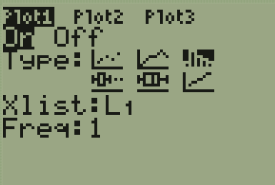
\includegraphics[width=2in]{calculatorHistogram}
\end{center}

Notice the options you're given: \texttt{Xlist} and \texttt{Freq}.  The first option is asking for the list where you entered the data you want to graph.  The second is a bit trickier; you have two options.

\paragraph{Option 1:} Enter the raw data, writing every value in your data list into \texttt{L1}, and leave the frequency option as 1, meaning that every value you've listed appears once.  In this case, the calculator will count the frequencies for you.

\paragraph{Option 2:} If you have a frequency table already built, you can enter that in the calculator; write the values in \texttt{L1} and the frequencies in \texttt{L2}.  Then write \texttt{L2} in the option for \texttt{Freq} in this menu (to write \texttt{L2}, press \calcbutton{2ND} then \calcbutton{2}).

Once you've entered the data and selected the appropriate options, pressing \calcbutton{GRAPH} will open the graphing window.
\pagebreak

\paragraph{NOT SO FAST!} If you press \calcbutton{GRAPH} now, you may see an empty graph.  The reason is that the window is not necessarily set to the right parameters.  Press the \calcbutton{WINDOW} button.
\begin{center}
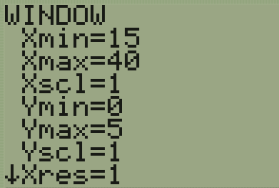
\includegraphics[width=2in]{calculatorHistogramWindow}
\end{center}

Most of the values are what you would expect: \texttt{Xmin} and \texttt{Xmax} define the lower and upper bounds of the horizontal axis, so we've set them to 15 and 40, respectively, to make sure that we can see all the results.  The options for \texttt{Ymin} and \texttt{Ymax} are similar; it may take some trial and error to set the upper bound, since we don't know the max frequency before graphing.\\

The one that is not as obvious is that \texttt{Xscl} does more than set the distance between grid marks.  For a histogram, this actually defines the \textbf{class width}, so if we wanted a grouped histogram, we would simply need to change this value.

In our example, though, we won't use any grouping, so we can now graph the histogram.
\begin{center}
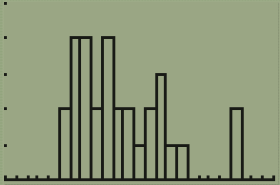
\includegraphics[width=2in]{calculatorHistogramGraph}
\end{center}

As it is, the histogram gives us the visual display of the data, but it's hard to read the actual frequencies.  However, if you press the \calcbutton{TRACE} button, you can use the arrow keys to navigate from one bar to the next, seeing the frequency for each.
\begin{center}
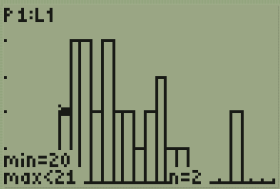
\includegraphics[width=2in]{calculatorHistogramTrace}
\end{center}
In this case, we've selected the bar ``between'' 20 and 21; really, this means anyone at 20 years old.  Notice on the lower right the value of \texttt{n} is 2, which is the frequency for this category.

\subsubsection{Scatterplots}
Drawing a scatterplot on the calculator is simpler; we only have to enter the values of $x$ in \texttt{L1} and $y$ in \texttt{L2}, then adjust the window to ensure that all the points are visible.  The scatterplot for the example comparing points per game and salary is shown below.
\begin{center}
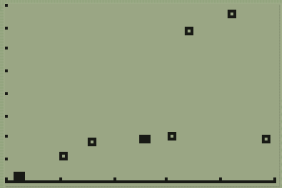
\includegraphics[width=2in]{calculatorScatterplotGraph}
\end{center}
The low resolution on the calculator makes it hard to see, but there are a few overlapping points; the general trend, though, is visible.
\pagebreak

\subsection{Using Excel}
\subsubsection{Histograms}
To draw a histogram in Excel, the data must be arranged in a frequency table to begin (there are ways to get Excel to build a frequency table from raw data, but these are too complicated to show here).  For example, let's use the age data from the NBA dataset.
\begin{center}
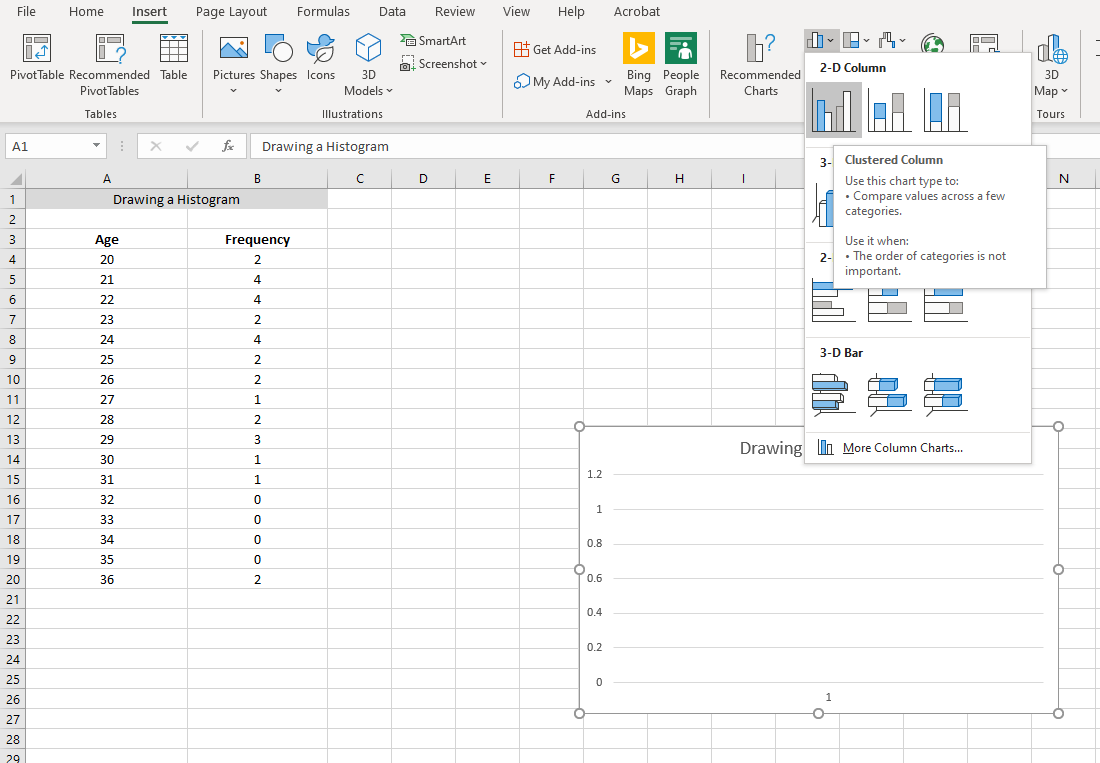
\includegraphics[height=2.5in]{ExcelHistogram1}
\end{center}
After entering the data, select the Insert tab along the top menu, and choose the first type of bar chart listed.  When you do, Excel may try to guess what data you're trying to use, but it probably won't guess correctly.

Right-click on the graph and choose the ``Select Data...'' option.  If there are any data series automatically added, remove them.
\begin{center}
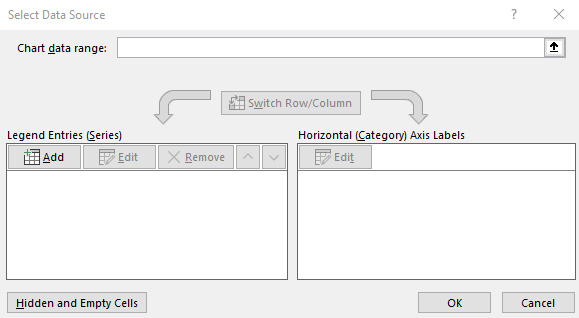
\includegraphics[height=1.25in]{ExcelHistogram2}
\end{center}
Now click on the Add button.  The series name is optional, but delete the series values, and with that field selected, click and drag to select the \emph{frequencies}.
\begin{center}
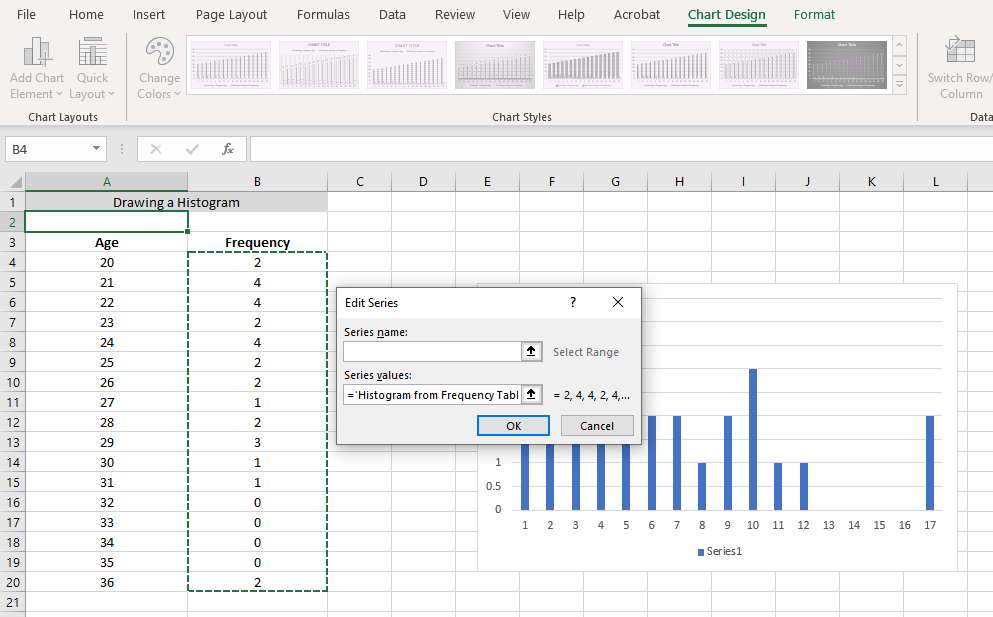
\includegraphics[height=2.5in]{ExcelHistogram3}
\end{center}

Notice that the graph so far shows the correct heights for the bars, but the horizontal axis labels are wrong.  To fix this, we need to edit the ``Horizontal (Category) Axis Labels'' on the right of the Data Source menu.
\begin{center}
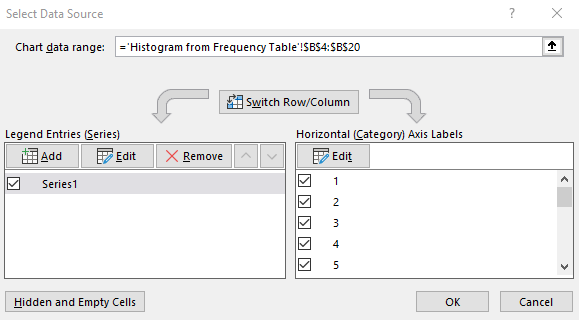
\includegraphics[height=1.25in]{ExcelHistogram4}
\end{center}
When you select Edit, it will open a dialog that allows you to select the cells for the labels.  Select the data in the age column.
\begin{center}
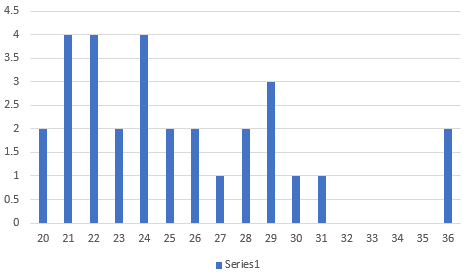
\includegraphics[height=1.25in]{ExcelHistogram5}
\end{center}

At this point, the graph is almost completed, but the bars are separated, and since this is a histogram (numerical data) instead of a bar chart (categorical data), we don't want a gap between them.  To fix this, right-click on one of the bars and select the option labeled ``Format Data Series.'' In the menu that opens to the right, find the option called ``Gap Width,'' and change this to 0\%.
\begin{center}
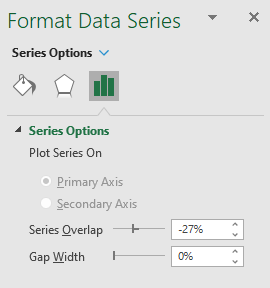
\includegraphics[height=1.7in]{ExcelHistogram6}
\end{center}

There are other small, optional options you can adjust, like adding axis and chart titles and removing the legend.  Also, it can be helpful to add borders to the bars (in the same Format Data Series menu).

Here's the final histogram:
\begin{center}
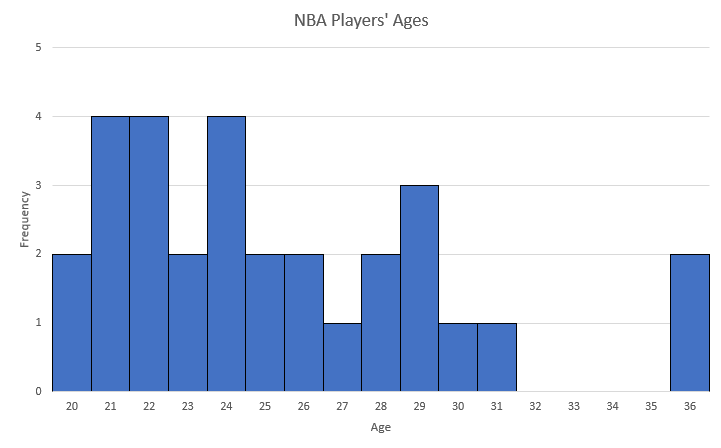
\includegraphics[height=2.5in]{ExcelHistogram7}
\end{center}
\pagebreak

\subsubsection{Scatterplots}
Thankfully, it is much easier to create a scatterplot using Excel.  With the data arranged in columns for $x$ and $y$, simply select the data, and insert a chart; select the first option under ``Scatter.''
\begin{center}
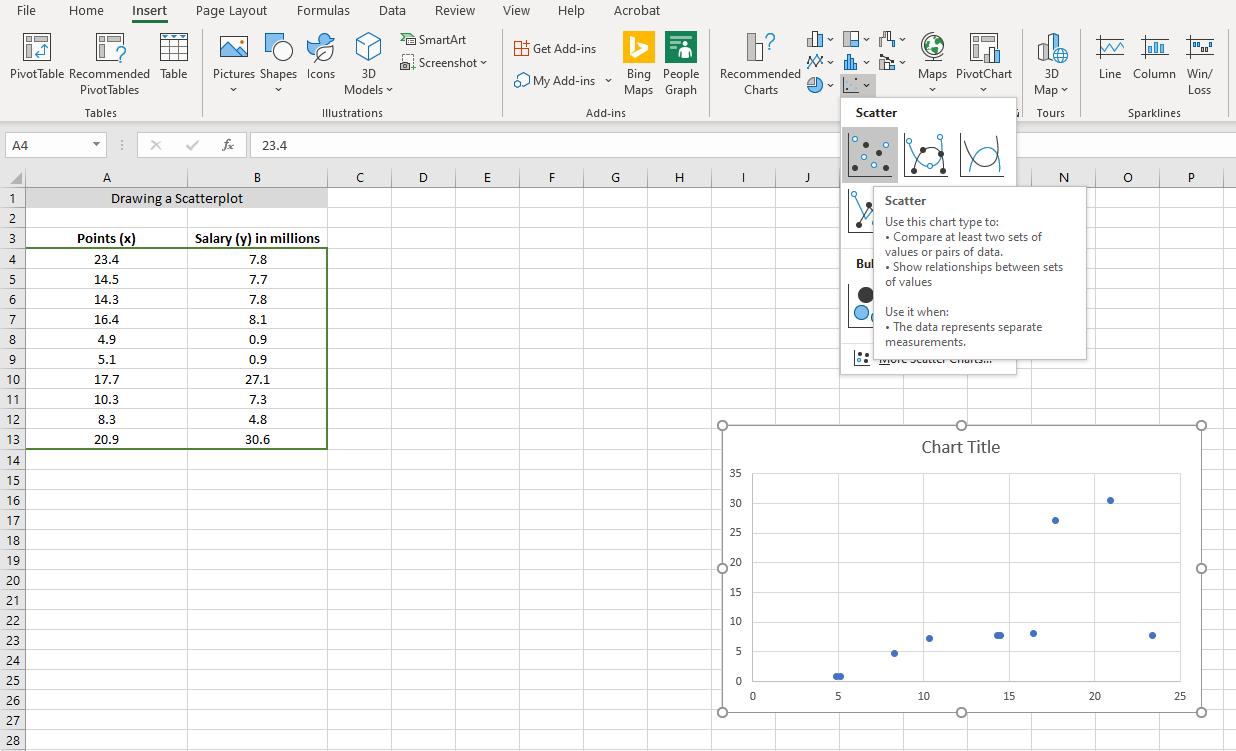
\includegraphics[height=3in]{ExcelScatterplot1}
\end{center}

After adding the chart and axis titles, here's the result:
\begin{center}
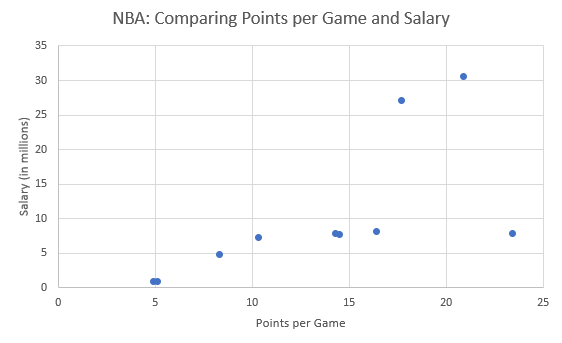
\includegraphics[height=2.5in]{ExcelScatterplot2}
\end{center}